\chapter{Теоретический базис} \label{chapt1}
В настоящей главе будут разобраны элементы статистической оптики, а именно одна из основных теорем статистической оптики, теорема Ван Циттерта - Цернике. Используя вывод теоремы, в качестве примера, оценивается пятно когерентности излучения для рентгеновской трубки -- полностью некогерентного источника излучения, и далее даётся формулировка обобщённой теоремы Ван Циттерта - Цернике в случае, когда на источнике излучения есть конечная область когерентности, или другими словами источник частично когерентен. Так же в главе рассматриваются вопросы формирования синхротронного излучения от электронного пучка с конечным эмиттансом. Обсуждаются статистические свойства такого излучения и описывается характерная спайковая структура излучения для одной статистической реализации поля.
\section{Распространение функции взаимной когерентности и теорема Ван Циттерта - Цернике}
Распространение функции взаимной когерентности~\ref{eq:g1} поля $E(r, t)$ через свободное пространство от некогерентных стационарных источников излучения описывается теоремой Ван Циттерта - Цернике \cite{van_cittert_wahrscheinliche_1934}, \cite{zernike_concept_1938}. 
\begin{align}
	\Gamma^{(1)} (r_1, r_2, t) = \cfrac{\big \langle {E}(r_1, t) {E}(r_2, t) \big \rangle}{\big \langle {E}(r_1, t)\big \rangle \big \langle{E}(r_2, t) \big \rangle}, 
	\label{eq:g1} 
\end{align}
где $\big \langle ... \big \rangle$ означает усреднение по статистическим реализациям поля. Теорема даёт связь между распределением интенсивности источника излучения $I(\xi, \eta)$ и функцией взаимной когерентности $\Gamma^{(1)} (r_1, r_2, t)$ через двумерное Фурье преобразование
\begin{align}
	\Gamma^{(1)} (r_1, r_2, t) = \cfrac{\kappa e^{-i\psi}}{(\bar{\lambda}z)^2} \iint \limits_{-\infty}^{+\infty} I(\xi, \eta) \exp{\big [(i \cfrac{2 \pi}{{\lambda}z}) (\Delta x \xi + \Delta y \eta)\big]}d\xi d\eta, 
	\label{eq:van_cittert_zernike_theorem} 
\end{align}
где $\kappa = {\lambda}^2 / \pi$, ${\lambda}$ -- длина волны монохроматического источника излучения\footnote{В оригинальной работе теорема формулируется для квазимонохроматического источника. Для простоты мы опускаем эту общую формулировку и сужаем теорему для монохроматических источников}, $z$ -- расстояние до плоскости наблюдения от источника излучения, $\psi = \cfrac{\pi}{\bar{\lambda} z}\big[((x^2_2 + y^2_2) - (x^2_1 + y^2_1)) \big]$, а $\Delta x = x_2 - x_1$, $\Delta y = y_2 - y_1$, другие геометрические величины изображены на Рис.~\ref{fig:VCC_scheme_incoh} 
\begin{figure}[H] 
	\centering 	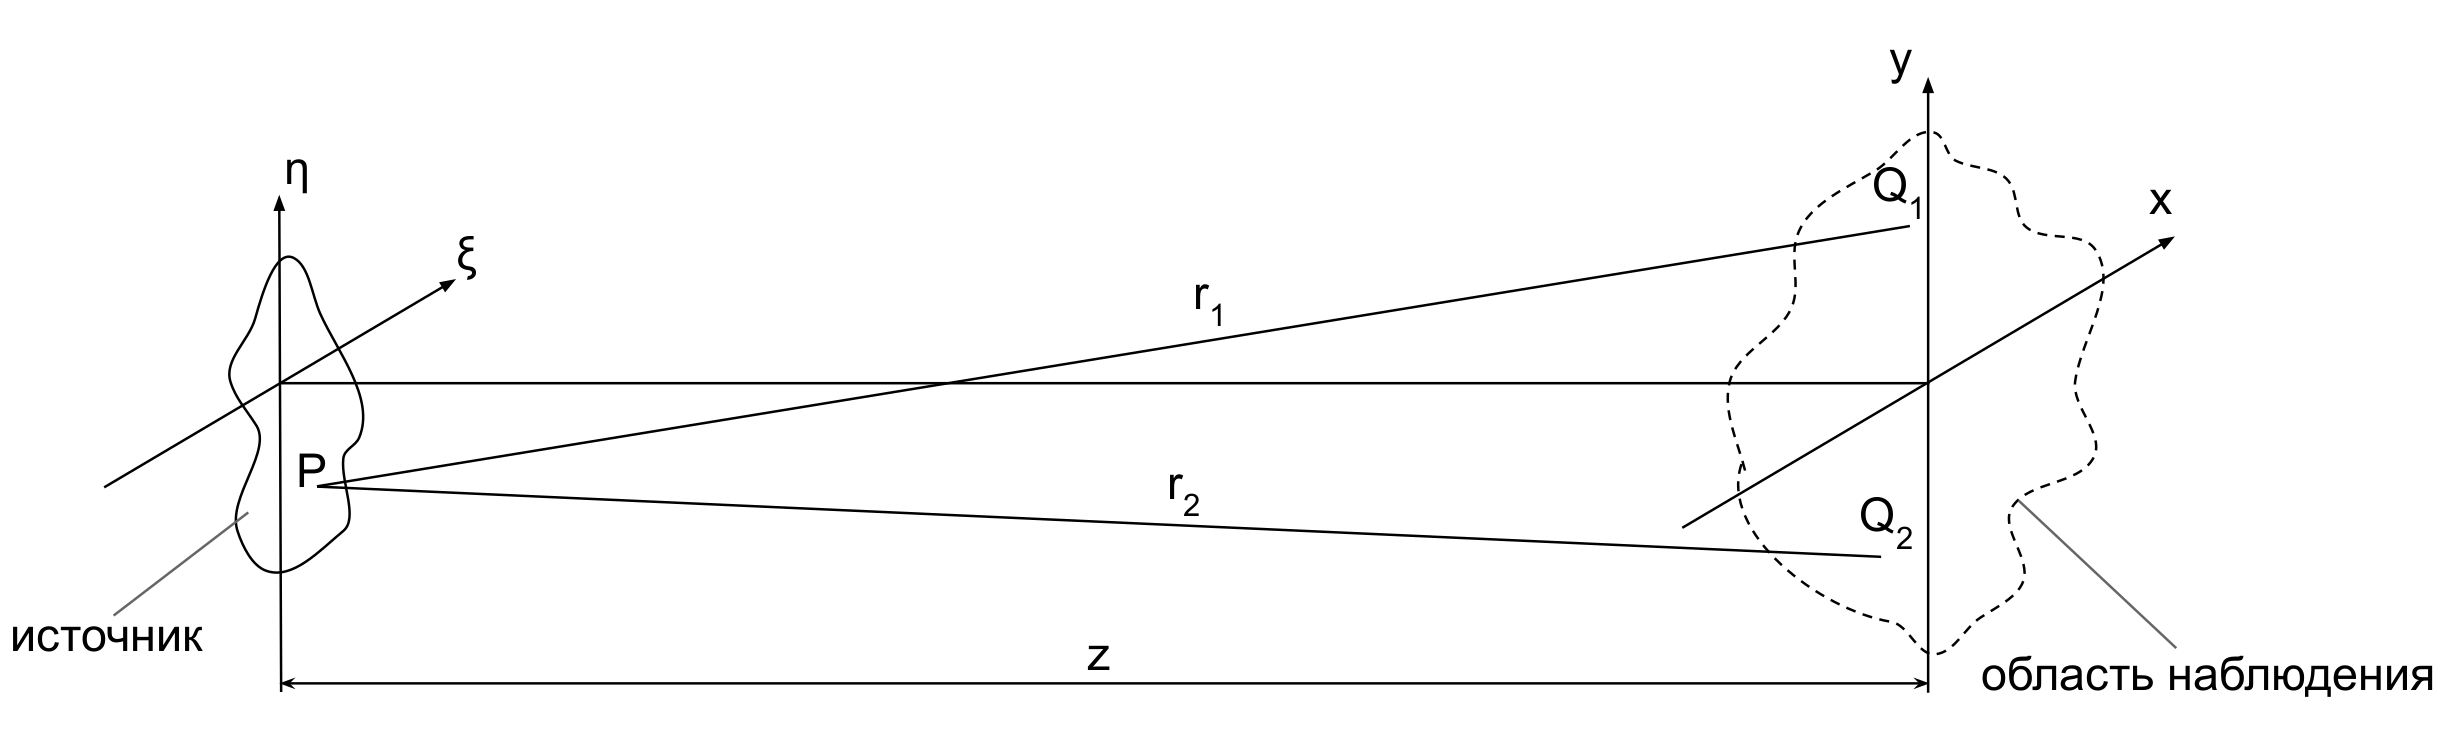
\includegraphics[width=0.99\linewidth]{VCC_incoh_scheme.png}
	\caption{К формулировке теоремы Ван Циттерта-Цернике}
	\label{fig:VCC_scheme_incoh}
\end{figure}
Таким образом площадь пятна когерентности на расстоянии $z$ от источника будет определяться следующим выражением
\begin{align}
	A_c = \cfrac{({\lambda} z)^2}{A_s}.
	\label{eq:VCC}
\end{align}

Теорема может быть видоизменена и обобщена для частично когерентных источников излучения достаточно лишь заменить $\kappa$ на двойной интеграл \cite{goodman_statistical_2015}
\begin{align}
	\kappa(\bar{x}, \bar{y}) = \iint \limits_{-\infty}^{+\infty} \mu(\Delta \xi, \Delta \eta) \exp{\big [(i \cfrac{2 \pi}{\bar{\lambda}z}) ( \bar{x} \Delta \xi + \bar{y} \Delta \eta)\big]}d\Delta \xi d\Delta \eta, 
\end{align}
где $\bar{x} = \cfrac{x_1 + x_2}{2}, \bar{y} = \cfrac{y_1 + y_2}{2}$,  $\Delta \xi = \xi_2 - \xi_1$, $\Delta \eta = \eta_2 - \eta_1$ и $\mu(\Delta \xi, \Delta \eta)$ -- комплексный коэффициент когерентности, по сути, область когерентности на источнике. Физически это значит следующее, Рис.~\ref{fig:VCC_scheme_partially}: огибающая излучения в дальней зоне будет обратно пропорциональна пятну когерентности излучения на источнике, а характерный размер когерентности в плоскости $xy$ на расстоянии $z$ обратно пропорционален размеру источника излучения -- интегральный множитель в формуле~\ref{eq:van_cittert_zernike_theorem}.
\begin{figure}[H] 
	\centering 	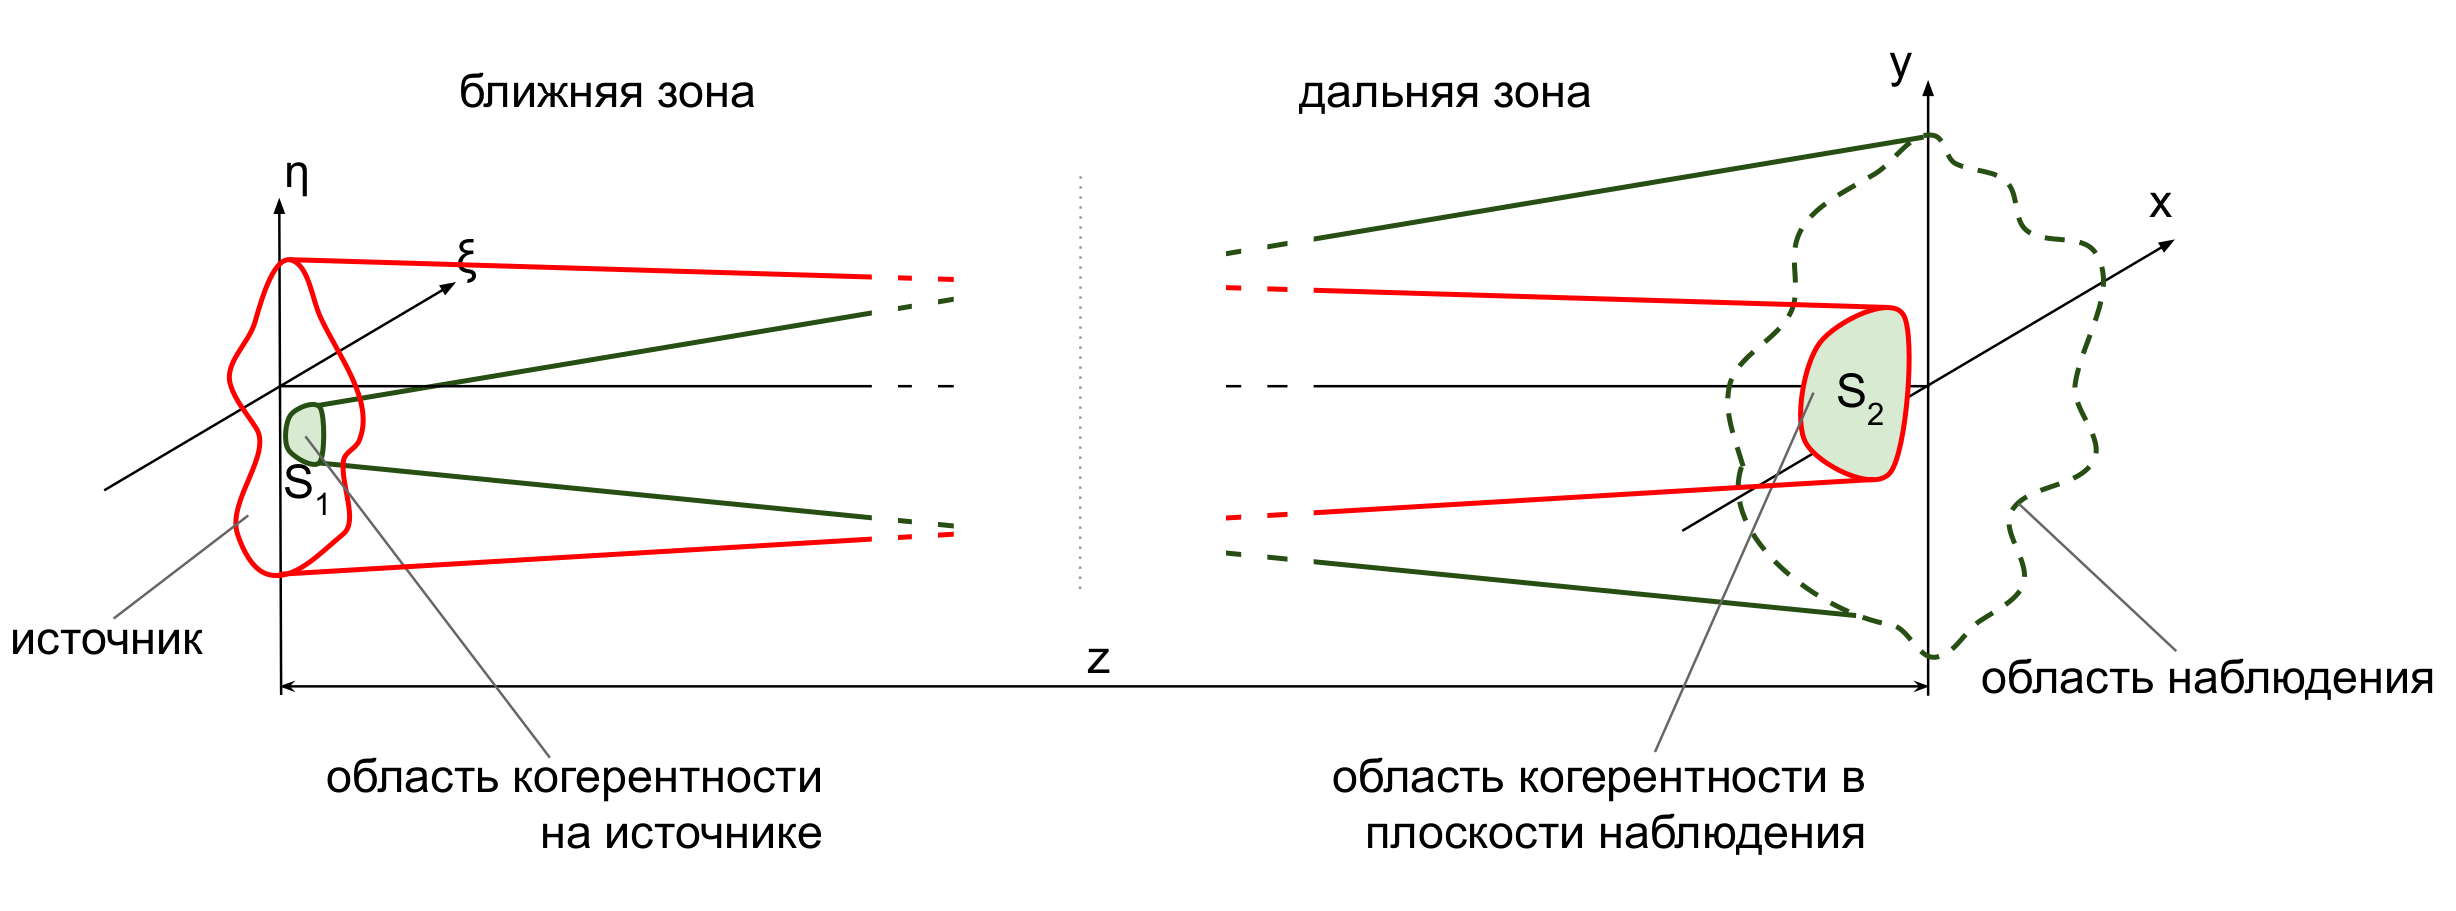
\includegraphics[width=0.99\linewidth]{VCC_partially_coh_scheme.png}
	\caption{К формулировке теоремы Ван Циттерта-Цернике}
	\label{fig:VCC_scheme_partially}
\end{figure}

В качестве примера распространения когерентности от полностью некогерентного источника можно оценить область когерентности излучения лабораторной рентгеновской трубки на некотором расстоянии $z$. Область когерентности от полностью некогерентного источника излучения квадратной формы получается напрямую из теоремы Ван Циттерта - Цернике. Подставляя в уравнение~\ref{eq:VCC} $z = 1$ м и $\lambda \approx 0.7$ $\textup{\AA}$ и площадью фокального пятна, спроецированного на направление выхода излучения из рентгеновской трубки, равной порядка $A_s = 1$ $\textup{мм}^2$, \cite{cullity_elements_1956}. Таким образом линейный размер длины когерентности при отражении от исследуемого кристалла с учётом угла дифракции ($\sim 45^{\circ}$) будет порядка $0.1$ $\textup{мкм}$. Однако линейный размер пятна когерентности может быть увеличен до нескольких микрон при использовании трубки с вращающимся анодом, где характерный размер источника достигает $50$ $\textup{мкм}$ \cite{cullity_elements_1956}.  

Для синхротронных источников излучения область когерентности на источнике определяется натуральным размером излучения одного электрона при пролёте через вставное устройство. Например, в случае ондуляторного источника, натуральный размер излучения определяется геометрическим размером перетяжки излучения в центре ондулятора -- $\sigma_r = \sqrt{\lambda L}/4 \pi$, где $L$ длина ондулятора. Дальнейшие рассуждения о статистических свойствах синхротронного представлены в следующем разделе, а точные выражения представлены в~\cite{geloni_transverse_2008}. 

\section{О статистических свойства синхротронного излучения}
Излучение от всего электронного пучка может быть представлено как сумма полей от каждого электрона, где $k$-ый электрон в пучке имеет свою координату -- $\vec{\eta}_k$, угол -- $\vec{\l}_k$, отсчитываемые от проектной траектории, а также время прибытия $t_k$ относительно некоторого времени $t_0$. Ондуляторное излучение удобно рассматривать в $\omega$-пространстве, т.е. $\bar{E}(\vec{r}, \omega)$, которое связано с полем $E(r, t)$ обратным преобразование Фурье по временной переменной. Вклад времени прибытия в $r\omega$-пространстве будет простым умножением поля на фазовый фактор $\exp{(i \omega t_k)}$. Указанные величины $\vec{\eta}_k$, $\vec{\l}_k$ и $t_k$ подчиняются некоторым распределениям плотности вероятности, для накопительных колец в модельных случаях это распределение Гаусса. В настоящей работе не рассматриваются эффекты, связанные с влияние разброса электронов по энергии на когерентные свойства излучения, эти эффекты описаны в \cite{geloni_effects_2018}. 

Результирующее поле от $N_e$ электронов на расстоянии $z$ от источника можно записать следующим образом:
\begin{align}
	\bar{E}_{b} (z, \vec{r}, \omega) = \sum\limits_{k=1}^{N_e} \bar{E}(\vec{\eta}_k, \vec{\l}_k, z, \vec{r}, \omega) \exp{(i \omega t_k)},
	\label{eq:E_bunch} 
\end{align}
для электронов в накопительных кольцах случайные величины $\vec{\eta}_k$ и $\vec{\l}_k$ не зависят от времени прибытия $t_k$ и, в центре ондулятора, независимы друг от друга. Модуль поля $|\bar{E}_k|$ имеет одинаковое распределение для всех $k$ со средним $\big \langle|\bar{E}_k|\big \rangle$ и конечным вторым моментом  $\big \langle|\bar{E}_k|^2\big \rangle$, где -- $\langle \cdot \rangle$ усреднение по статистическим реализациям.

Результирующее монохроматическое поле $\bar{E}_{b}$ является суммой вкладов от каждого электрона в пучке и по своей структуре в правой части уравнения~\ref{eq:E_bunch} записан некоторый фазор. Следуя предпосылкам центральной предельной теоремы (ЦПТ), можно показать, что поле $\bar{E}_{b}(z, \vec{r}, \omega)$ в каждой точке $\vec{r}$ подчиняется комплексному гауссовому распределению для двух практически значимых предельных случаев: случай «длинного» $\omega\sigma_T \gg 1$ и «короткого»  $\omega\sigma_T \ll 1$ электронного пучка, где $\sigma_T$ -- длительность электронного пучка. В случае длинного электронного пучка величина $\omega t_k$ равномерно распределена в пределах от $0$ до $2\pi$ и продольная длина когерентности излучения на фундаментальной гармонике определятся натуральной длительностью излучения от одного электрона $c/\lambda N_w = \omega / N_w$, где $N_w$ количество периодов ондулятора, которая также в большинстве практических случаях в рентгеновском диапазоне длин волн много меньше длительность электронного импульса. Этот случай будет, для определённости, называться продольно некогерентным. Для короткого электронного пучка фазовый множитель $\exp{(i \omega t_k)}$ может быть взят равным единице и излучение является продольно когерентным. В целом, формула~\ref{eq:E_bunch} даёт прямой путь моделирования синхротронного излучения с любой степенью когерентности, с учётом продольной когерентности/некогрентности излучения.

Как уже было отмечено амплитуда поля по формуле~\ref{eq:E_bunch} обладает спайковой структурой, и, что важно отметить, как в $\omega t$-пространстве, так и в поперечном направлении в $rk$-пространстве. В итоге, получается некая трёхмерная структура, изображённая на Рис.~\ref{fig:spikes}, с флуктуирующей амплитудой поля. 
\begin{figure}
	\centering 	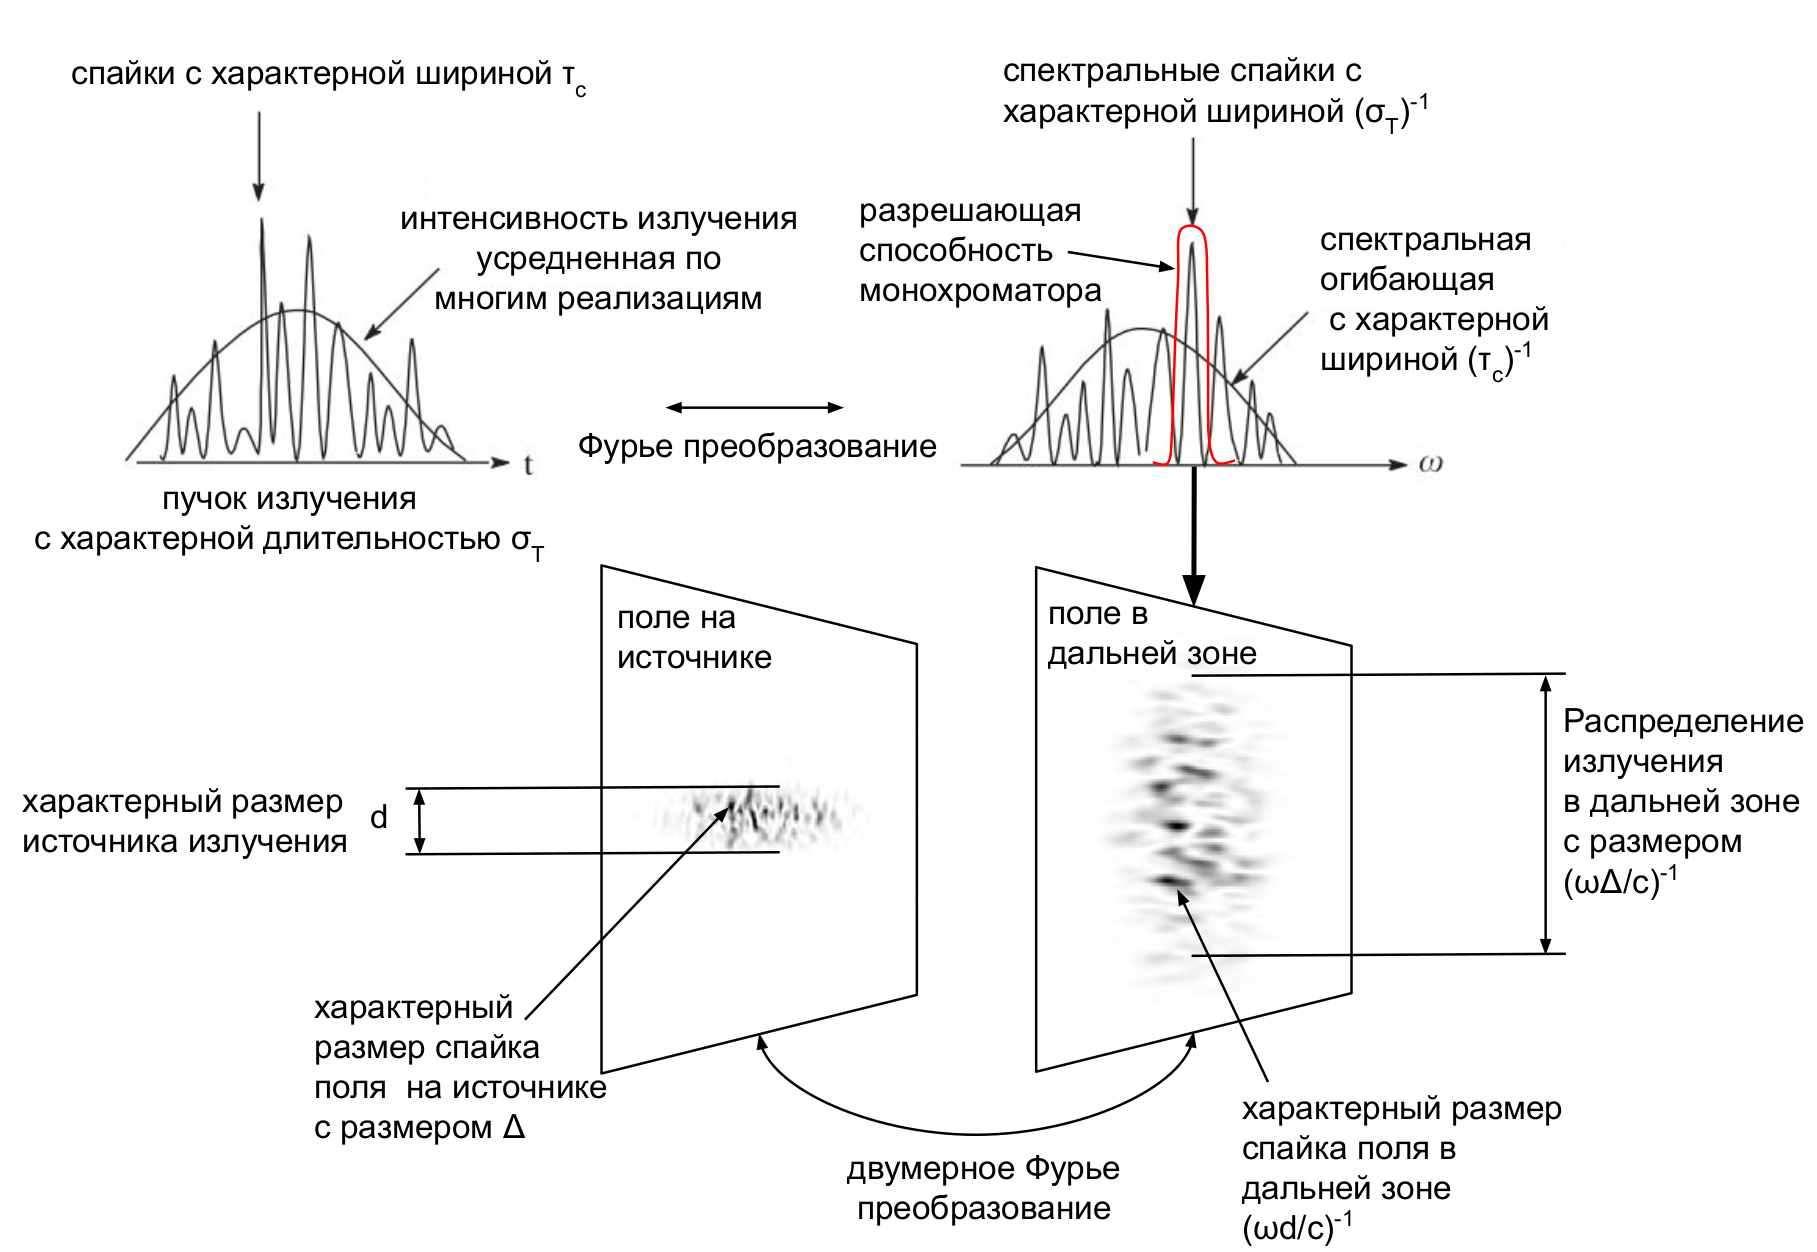
\includegraphics[width=0.99\linewidth]{spikes.png}
	\caption{Спайковая структура излучения синхротронного излучения.}
	\label{fig:spikes}
\end{figure}

В $t$-пространстве поле имеет внутреннюю структуру с характерным размером спайка равному продольной длине когерентности излучения от одно электрона, а характерная длительность импульса поля, усреднённого по многим реализациям, определяется длительностью электронного пучка. В виду связи $\omega t$-пространств, в $\omega$-пространстве размер спайка в спектре обратно пропорционален длительности излучения, а характерная огибающая спектра, после усреднения по многим реализациям, обратно пропорциональна длине когерентности излучения, такое соотношение -- следствие теоремы Винера-Хинчина. Если разрешить монохроматором (красная линия на Рис.~\ref{fig:spikes}) спайк в $\omega$-пространстве, то на двумерном детекторе в дальней зоне можно увидеть поперечную спайковую структуру синхротронного излучения, как на Рис.~\ref{fig:spikes}. Это распределение с точностью до фазового фактора связано с распределением излучения на образце Фурье-преобразованием. В дальней зоне характерный размер спайка связан с размером источника излучения как:  $(\omega d /c)^{-1}$, и огибающая поля -- усреднённое по многим реализациям: $(\omega \Delta /c)^{-1}$, -- что является следствием обобщённой теоремы Ван Циттерта - Цернике. 


\newpage
%============================================================================================================================






